\documentclass[11pt]{article}
\usepackage[utf8]{inputenc}
\usepackage[T1]{fontenc}
\usepackage{lmodern}
\usepackage{geometry}
\usepackage{tikz}
\usetikzlibrary{arrows.meta,shapes.geometric}

\geometry{paperwidth=16cm,paperheight=6.9cm,margin=0cm}
\pagestyle{empty}
\setlength{\parindent}{0pt}

\definecolor{ctxFill}{RGB}{238,242,245}
\definecolor{ctxLine}{RGB}{155,168,179}
\definecolor{ctxText}{RGB}{38,52,67}
\definecolor{exFill}{RGB}{220,233,247}
\definecolor{exLine}{RGB}{23,54,93}
\definecolor{prFill}{RGB}{200,240,236}
\definecolor{prLine}{RGB}{8,127,140}
\definecolor{prText}{RGB}{6,79,87}
\definecolor{phFill}{RGB}{234,242,245}

\begin{document}
\noindent
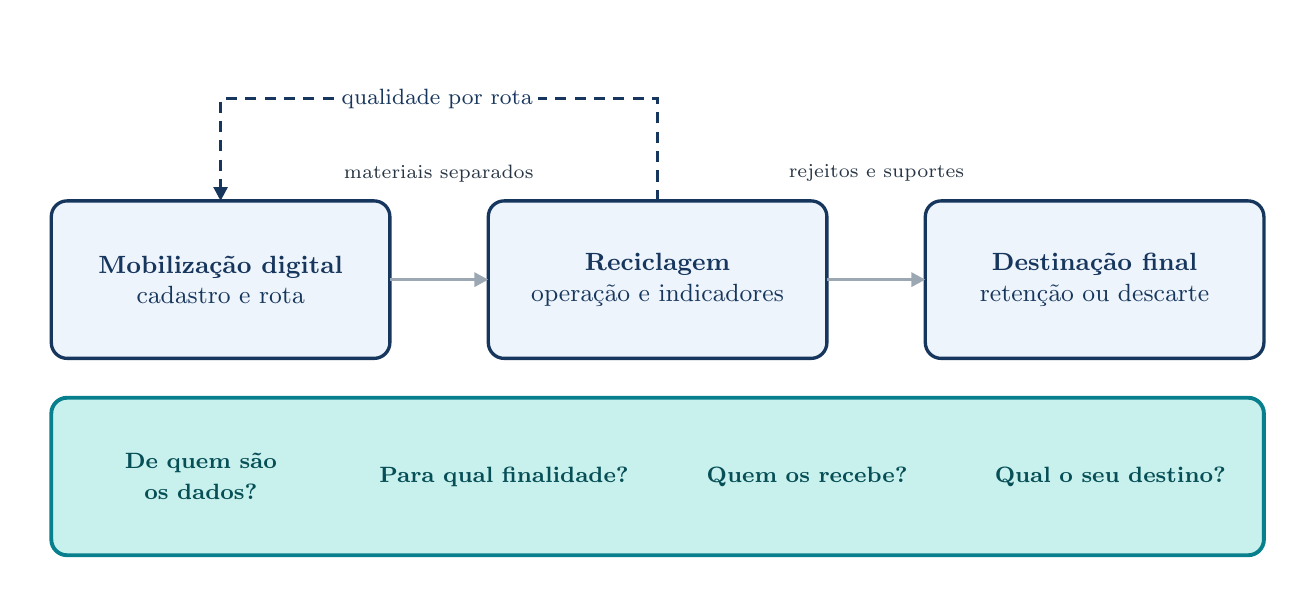
\begin{tikzpicture}[x=1cm,y=1cm,font=\small]
  \path[use as bounding box] (0,0) rectangle (16,6.9);
  \draw[fill=exFill!50,draw=exLine,line width=1.2pt,rounded corners=0.2cm] (0.3,2.7) rectangle (4.6,4.7);
  \node[align=center,text=exLine] at (2.4499999999999997,3.7) {\textbf{Mobilização digital}\\ cadastro e rota};
  \draw[fill=exFill!50,draw=exLine,line width=1.2pt,rounded corners=0.2cm] (5.85,2.7) rectangle (10.149999999999999,4.7);
  \node[align=center,text=exLine] at (8.0,3.7) {\textbf{Reciclagem}\\ operação e indicadores};
  \draw[fill=exFill!50,draw=exLine,line width=1.2pt,rounded corners=0.2cm] (11.4,2.7) rectangle (15.7,4.7);
  \node[align=center,text=exLine] at (13.55,3.7) {\textbf{Destinação final}\\ retenção ou descarte};
  \draw[draw=ctxLine,line width=1.2pt,-{Triangle[length=5pt,width=5pt]}] (4.6,3.7) -- (5.85,3.7);
  \draw[draw=ctxLine,line width=1.2pt,-{Triangle[length=5pt,width=5pt]}] (10.15,3.7) -- (11.4,3.7);
  \node[text=ctxText,align=center] at (5.22,5.05) {\scriptsize materiais separados};
  \node[text=ctxText,align=center] at (10.78,5.05) {\scriptsize rejeitos e suportes};
  \draw[draw=exLine,line width=1.1pt,dash pattern=on 4pt off 3pt,-{Triangle[length=5pt,width=5pt]}] (8.0,4.7) -- (8.0,6.0) -- (2.45,6.0) -- (2.45,4.7);
  \node[text=exLine,fill=white,inner sep=2pt] at (5.2,6.0) {\footnotesize qualidade por rota};
  \draw[fill=prFill,draw=prLine,line width=1.4pt,rounded corners=0.2cm] (0.3,0.2) rectangle (15.7,2.2);
  \node[text=prText,align=center,text width=3.4cm] at (2.2,1.2) {\footnotesize\textbf{De quem são os dados?}};
  \node[text=prText,align=center,text width=3.4cm] at (6.050000000000001,1.2) {\footnotesize\textbf{Para qual finalidade?}};
  \node[text=prText,align=center,text width=3.4cm] at (9.9,1.2) {\footnotesize\textbf{Quem os recebe?}};
  \node[text=prText,align=center,text width=3.4cm] at (13.75,1.2) {\footnotesize\textbf{Qual o seu destino?}};
\end{tikzpicture}
\end{document}
